\documentclass[11pt, a4paper, oneside, chapter, romanfixed]{oblivoir}

% Preamble
\usepackage{listings}           % 코드 구문 삽입을 위함
\usepackage{xcolor}             % 글자색 조정
\usepackage{tikz, blindtext}    % 그래픽 chapter 사용을 위함
\usepackage{graphicx}           % 그래픽(사진) 삽입을 위함
\usepackage{fapapersize}        % 조판 종이 설정
\usepackage{hyperref}           % href 설정
\usepackage{kotex}              % 한글 설정을 위함
\usepackage{tabu}               % 쉬운 table 그리기
\usepackage{float}              % 테이블 위치를 결정하기 위함

% Preamable - 여백 조정
\usefapapersize{*,*,30mm,*,30mm,*}

% Preamable - Chapter 스타일 설정
\makechapterstyle{box}{
  \renewcommand*{\printchaptername}{}
%   \renewcommand*{\chapnumfont}{\normalfont\sffamily\huge\bfseries}
  \renewcommand{\prechapternum}{}       % 한국어 매크로 제거를 위함 '제'
  \renewcommand{\postchapternum}{}      % 한국어 매크로 제거를 위함 '장'
  \renewcommand*{\printchapternum}{
    \flushright
    \begin{tikzpicture}
      \draw[fill,color=black] (0,0) rectangle (2cm,2cm);
      \draw[color=white] (1cm,1cm) node { \chapnumfont\thechapter };
    \end{tikzpicture}
  }
%   \renewcommand*{\chaptitlefont}{\normalfont\sffamily\Huge\bfseries}
  \renewcommand*{\printchaptertitle}[1]{\flushright\chaptitlefont##1}
}
\chapterstyle{box}

% https://texblog.org/2012/07/03/fancy-latex-chapter-styles/
% http://ajt.ktug.org/2011/0501karnes.pdf


% Preamable - href 설정
\hypersetup{
    colorlinks=true,
    linkcolor=black,    % 목차 href는 검은색
    filecolor=magenta,      
    urlcolor=blue,      % 외부 url이 포함된 href는 파란색
    pdfpagemode=FullScreen,
}


% Preamble - code style 설정
\lstset{
  basicstyle=\ttfamily\small,
  commentstyle=\color{green},
  keywordstyle=\color{blue},
  stringstyle=\color{red},
  breaklines=true,
  frame=single,
  language=bash,
  showstringspaces=false
}

\pagestyle{plain}


% Body
\begin{document}

\title{모던 리눅스 교과서 1주차}
\author{최우성}
\date{ }
\maketitle
\newpage


\tableofcontents

\chapter{리눅스 소개}

\section{모던 환경이란 무엇인가?}
작성 시점인 2024년 기준 리눅스는 다양한 환경에서 사용된다.

\begin{itemize}
    \item 모바일 디바이스 \newline 
        안드로이드 OS는 리눅스의 변형이다.
    \item 클라우드 컴퓨팅 \newline  
        리눅스는 CSP에서 제공하는 서버의 OS로 많이 사용된다.
    \item IoT \newline
        리눅스는 사물 인터넷 OS로도 사용된다.
    \item 프로세스 아키텍처의 다양성 \newline 
        전통의 x86-64 이외에도 ARM, RSIC-V 같은 ISA도 지원된다.
    \item 컨테이너 인프라 \newline
        Kubernetes, Docker로 대표되는 컨테이너 인프라에서 기본적으로 사용된다.
\end{itemize}
\newpage


\section{리눅스 역사}
\subsection*{90년대}
1991년 리누스 토르발스에 의해 시작되었으며 수많은 기여자의 도움으로 리눅스 1.0.0은 3년이 되기도 전에 릴리즈되었다.
\newline
이 시점에서 Unix/GUN 소프트웨어를 실행할 수 있는 운영체제라는 최초 목표는 달성되었다.
또한, 이 기간에 최초의 상용 리눅스인 Red Hat 리눅스가 등장했다.

\subsection*{2000 - 2010}
여러 기업에서 리눅스를 본격적으로 도입하며 폭팔적으로 성장하는 시기이다.\newline
이 시기부터 Linux는 Unix, Windows Server 같은 경쟁 서버보다 점유율 우위를 점하기 시작한다.
또한, 여러 배포판(distro)가 출시되며 경쟁했다.

\subsection*{2010 이후}
단순 서버용 이상으로 확장되어 IoT, 모바일 디바이스에서도 사용한다.\newline
또한, 컨테이너 인프라가 본격적으로 사용되기 시작했다.\newline
그리고, 상용 서버 배포판은 사실상 Red Hat, Debian 기반으로 수렴했다.

\begin{flushleft}
    보다 상세한 한글 자료는 \href{https://zdnet.co.kr/view/?no=20200826135027}{리눅스 29돌 사건으로 보는 그 역사}를 참고하라.    
\end{flushleft}



\section{리눅스 배포판}
\textbf{리눅스 커널}은 \textbf{단순 시스템 콜과 디바이스 드라이버의 집합}을 의미한다.\newline
\textbf{리눅스 배포판}은 \textbf{커널과 관련 구성요소의 전체 번들}을 의미한다. 
관련 구성요소에는 패키지 관리자, 파일시스템 레이아웃, init system, shell이 포함된다.
\newpage


\section{리소스 가시성}
리눅스는 리소스의 \textbf{전역 보기}(global view)를 지원한다.\newline
여기서 \textbf{전역보기}는 무엇이고 \textbf{전역보기의 반대}는 무엇이며 \textbf{리소스}는 무엇인가?

\subsection*{리소스란?}
\textbf{리소스}는 \textbf{소프트웨어 실행을 지원하는 데 사용할 수 있는 모든 것}으로 간주될 수 있다.\newline
예를 들면 다음과 같은 것이 리소스로 간주될 수 있다.

\begin{itemize}
    \item 하드웨어
    \item 파일시스템
    \item HDD/SSD
    \item process
    \item device
    \item routing table(Network)
    \item 자격증명(credential)
\end{itemize}

\subsection*{전역 리소스}
예를 들어 HDD 용량 확인, 특정 파일 읽기, ps -ef로 pid 확인하기 같은 것은 여러 계정에서 동일하게 볼 수 있다.
\newline
리눅스에서 할 수 있는 대부분의 것이 전역에서 되므로 리눅스의 모든 것은 전역일 것이라 기대할 수 있지만 
실제로 그렇지 않다.


\subsection*{로컬 리소스}
모든 리소스가 전역인 것은 아니다. 예를 들면 namespace를 통해 리소스의 로컬보기를 지원할 수 있다.
또한, 특정 프로세스가 메모리 리소스를 고갈시키는 것을 방지하기 위해 
메모리 소비를 제한하는 것도 메모리가 전역 리소스로 사용하지 않을 수 있다든 것을 보여준다.\newline
이처럼 리소스의 사용을 제한하는 것은 프로세스의 격리의 일종이며 
리눅스에서는 \textbf{cgoup}이라는 커널 기능을 사용해 이러한 종류의 격리를 제공한다.\newline

\chapter{리눅스 커널}
\section{리눅스 아키텍처}
\begin{itemize}
    \item \textbf{하드웨어 계층}\newline
        CPU와 메인 메모리, 디스크, NIC, I/O 디바이스 모두를 총칭한다.
    \item \textbf{커널 계층}\newline
        하드웨어 계층과 사용자 영역 계층의 사이에 위치한다.\newline
        이번 chapter에서 다루는 계층이다.
    \item \textbf{사용자 영역 계층}\newline
        shell 및 ps, ssh 같은 유틸리티, GUI를 비롯해 
        대부분의 앱이 실행되는 계층이다.
\end{itemize}

\begin{flushleft}
    다른 계층간 인터페이스는 리눅스 운영체제 패키지의 일부이다.
    그 중 커널과 사용자 영역 계층 인터페이스를 \textbf{시스템 콜}(system call)이라 부른다.
\end{flushleft}

\begin{flushleft}
    하드웨어와 커널 사이의 인터페이스는 시스템 콜과 달리 
    단일 인터페이스가 아니라 
    일반적으로 하드웨어별 그룹화된 개별 인터페이스 모음으로 구성된다.

    \begin{itemize}
        \item CPU 인터페이스
        \item main memory 인터페이스
        \item 네트워크 인터페이스와 드라이버
        \item 파일시스템과 블록 디바이스 드라이버 인터페이스
        \item 캐릭터 디바이스, 하드웨어 인터럽트, 
        키보드, 터미널, 기타 I/O 등의 입력 디바이스를 위한 디바이스 드라이버
    \end{itemize}
\end{flushleft}
\newpage

\begin{figure}
    \centering
    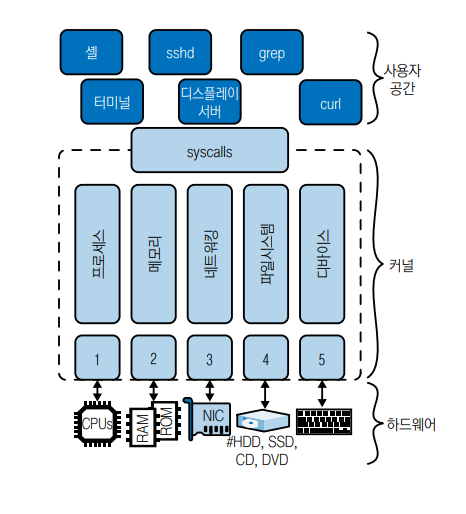
\includegraphics[width=10cm]{resource/2-1.png}
    \caption{리눅스 아키텍처 개요}
\end{figure}
\begin{flushleft}
    일반적으로 \textbf{커널 모드}는 추상화를 제한함으로써 빠르게 실행함을 의미하는 반면, 
    \textbf{사용자 모드}는 상대적으로 느리지만 더 안전하고 편리한 추상화를 의미한다.
    대부분의 경우 커널 모드를 신경쓰지 않아도 사용에 지장은 없지만, 
    커널과 상호 작용하는 방법(시스템 콜)을 아는 것은 중요하다.
\end{flushleft}


\section{CPU 아키텍처}
\subsection{x86-64 아키텍처}
\begin{flushleft}
    x86과 amd64를 합쳐서 x86-64라고 부른다. 
    x86은 인텔 32-bit ISA이며, amd64는 64-bit ISA이다.
    대부분의 경우 사용되는 CPU이며 오래전부터 사용되어왔고, 
    CISC(Complex Instruction Set Computer) 아키텍처 에너지 효율은 높지 않다.
\end{flushleft}

\subsection{ARM 아키텍처}
\begin{flushleft}
    RISC(Reduced Instruction Set Computer) 아키텍처이며 적은 명령어 집합을 사용한다.
    RISC는 CISC에 비해 전력 소모가 적다는 장점을 가지고 있으며, 
    저전력 환경(임베디드, 휴대용 디바이스)에서 널리 사용된다.
\end{flushleft}


\subsection{RISC-V 아키텍처}
\begin{flushleft}
    ARM과 달리 개방형 RISC 표준으로 아직 널리 사용되지는 않는다. 
    다만 ARM과 달리 라이센스 비용이 없어 주목받고 있다.
\end{flushleft}


\section{커널 구성요소}
커널 코드에서 제공하는 주요 기능은 다음과 같다.

\begin{itemize}
    \item \textbf{프로세스 관리}: 실행 파일을 기반으로 프로세스 시작
    \item \textbf{메모리 관리}: 프로세스에 메모리 할당 및 파일을 메모리에 매핑
    \item \textbf{네트워킹}: 네트워크 인터페이스 관리 및 네트워크 스택 제공
    \item \textbf{파일시스템}: 파일 관리를 제공하고, 파일 생성과 삭제 지원
    \item 케릭터 디바이스와 디바이스 드라이버 관리
\end{itemize}

\subsection{프로세스 관리}
\begin{itemize}
    \item \textbf{세션}\newline
        하나 이상의 프로세스 그룹을 포함하고 선택적으로 tty가 연결된 
        상위 수순의 사용자 대면 유닛.
        커널은 textbf{세션 ID}(SID)라는 번호를 통해 세션을 식별한다.
    \item \textbf{프로세스 그룹}\newline
        하나 이상의 프로세스가 포함되어 있으며, 
        한 세션에는 foreground 프로세스 그룹이 둘 이상일 수 없다.
        커널은 \textbf{프로세스 그룹 ID}(PGID)라는 숫자를 통해 프로세스 그룹을 식별한다.
    \item \textbf{프로세스}\newline
        여러 리소스(주소 공간, 하나 이상의 스레드, 소켓 등)를 그룹으로 추상화한 것이며, 
        커널은 /proc/self를 통해 현재 프로세스를 사용자에게 노출한다.
        커널은 \textbf{프로세스 ID}(PID)라는 숫자를 통해 프로세스를 식별한다.
    \item \textbf{스레드}\newline
        커널에 의해 프로세스로 구현된 유닛을 말한다.
        즉 스레드를 나타내는 전용 데이터 구조는 없다.
        오히려 스레드는 특정 리소스(ex - 메모리, signal handler)를 다른 프로세스와 공유하는 프로세스다.
        커널은 \textbf{스레드 ID}(TID)와 \textbf{스레드 그룹}(TGIO)를 통해 스레드를 식별하며, 
        공유된 TGID 값은 멀티스레드 프로세스를 의미한다.
    \item \textbf{태스크}\newline
        커널에는 sched.h에 정의된 \textbf{task\_struct}라는 데이터 구조가 있으며, 
        이는 프로세스와 스레드 구현의 기반을 형성한다.
        이 데이터 구조는 스케줄링 관련 정보, 식별자(ex - PID, TGID), signal handler, 
        성능이나 보안과 관련된 기타 정보를 수집한다.
        즉, 앞서 언급한 모든 유닛은 태스크에서 파생되거나 고정(anchor)된다. 
        하지만 캐스크는 커널 외부에 그대로 노출되는 일이 없다.
\end{itemize}

\begin{flushleft}
    실제로 그러한지 실습해보자.\newline
    아래는 ps -j로 확인할 수 있는 정보이다.
\end{flushleft}

\begin{figure}[h]
    \centering
    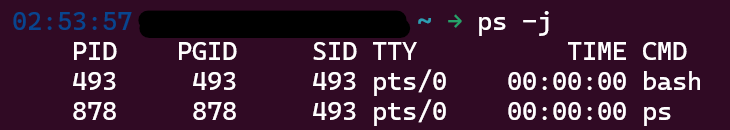
\includegraphics[width=10cm]{resource/ps-example.png}
    \caption{실습}
    \begin{enumerate}
        \item bash 셸 프로세스의 PID, PGID, SID는 모두 -이다.\newline
            ls -la /proc/493/task/493/로 태스트 수준의 정보를 수집할 수 있다.
        \item ps 프로세스의 PID/PGID는 878이고 SID는 셀과 동일하다.
    \end{enumerate}
\end{figure}

\begin{figure}
    \centering
    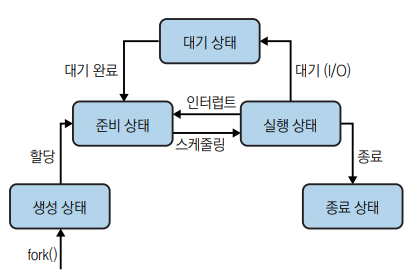
\includegraphics[width=10cm]{resource/2-2.png}
    \caption{리눅스 프로세스 상태}
\end{figure}


\subsection{메모리 관리}
작성예정

\subsection{네트워킹}
리눅스의 네트워크 스택은 계층화된 아키텍처를 따른다.

\begin{itemize}
    \item \textbf{소켓}\newline
        추상화 커뮤니케이션을 위해 필요
    \item \textbf{TCP(Transmission Control Protocol) 및 UDP(User Datagram Protocol)}\newline
        각각 연결형 통신과 비연결형 통신
    \item \textbf{인터넷 프로토콜}(IP)\newline
        기기의 주소 지정을 위해 필요
\end{itemize}

\begin{flushleft}
    이와 같은 세 가지 작업은 커널이 처리하는 모든 것이다.
    HTTP나 SSH 같은 애플리케이션 계층 프로토콜은 주로 사용자 영역에서 구현된다.
\end{flushleft}

\subsection{파일시스템}
\begin{flushleft}
    리눅스는 파일시스템을 사용해 HDD, SDD, 플래시 메모리 같은 
    저장 디바이스의 파일과 디렉터리를 구성한다. 
    ext4, btrfs, NTFS 같은 다양한 융형의 파일시스템이 있으며 
    동일한 파일 시스템의 인스턴스도 여러 개 사용할 수 있다.
\end{flushleft}
\begin{flushleft}
    가상 파일시스템(Virtual File System, VFS)은 원래 여러 파일시스템 유형과 인스턴스를 지원하기 위해 도입되었다.
    VFS의 최상위 계층은 열기, 닫기, 읽ㄱ, 쓰기 기능 등 공통 API 추상화를 제공하며, 
    VFS의 최하위 계층은 주어진 파일시스템에 대한 \textbf{플러그인}이라고 불리는 파일시스템 추상화다.
\end{flushleft}

\subsection{디바이스 드라이버}
작성 예정

\subsection{시스템 콜}
작성 예정

\section{커널 확장}
작성 예정

\subsection{모듈}
작성 예정

\subsection{커널을 확장하는 현대적인 방법: eBPF}
작성 예정
\end{document}
